%%%%%%%%%%%%%%%%%%%%%%%%%%%%%%%%%%%%%%%%%
% Arsclassica Article
% LaTeX Template
% Version 1.1 (1/8/17)
%
% This template has been downloaded from:
% http://www.LaTeXTemplates.com
%
% Original author:
% Lorenzo Pantieri (http://www.lorenzopantieri.net) with extensive modifications by:
% Vel (vel@latextemplates.com)
%
% License:
% CC BY-NC-SA 3.0 (http://creativecommons.org/licenses/by-nc-sa/3.0/)
%
%%%%%%%%%%%%%%%%%%%%%%%%%%%%%%%%%%%%%%%%%

%----------------------------------------------------------------------------------------
%	PACKAGES AND OTHER DOCUMENT CONFIGURATIONS
%----------------------------------------------------------------------------------------

\documentclass[
10pt, % Main document font size
a4paper, % Paper type, use 'letterpaper' for US Letter paper
oneside, % One page layout (no page indentation)
%twoside, % Two page layout (page indentation for binding and different headers)
headinclude,footinclude, % Extra spacing for the header and footer
BCOR5mm, % Binding correction
]{scrartcl}

%%%%%%%%%%%%%%%%%%%%%%%%%%%%%%%%%%%%%%%%%
% Arsclassica Article
% Structure Specification File
%
% This file has been downloaded from:
% http://www.LaTeXTemplates.com
%
% Original author:
% Lorenzo Pantieri (http://www.lorenzopantieri.net) with extensive modifications by:
% Vel (vel@latextemplates.com)
%
% License:
% CC BY-NC-SA 3.0 (http://creativecommons.org/licenses/by-nc-sa/3.0/)
%
%%%%%%%%%%%%%%%%%%%%%%%%%%%%%%%%%%%%%%%%%

%----------------------------------------------------------------------------------------
%	REQUIRED PACKAGES
%----------------------------------------------------------------------------------------

\usepackage[
nochapters, % Turn off chapters since this is an article        
beramono, % Use the Bera Mono font for monospaced text (\texttt)
eulermath,% Use the Euler font for mathematics
pdfspacing, % Makes use of pdftex’ letter spacing capabilities via the microtype package
dottedtoc % Dotted lines leading to the page numbers in the table of contents
]{classicthesis} % The layout is based on the Classic Thesis style

\usepackage{arsclassica} % Modifies the Classic Thesis package

\usepackage[T1]{fontenc} % Use 8-bit encoding that has 256 glyphs

\usepackage[utf8]{inputenc} % Required for including letters with accents

\usepackage{graphicx} % Required for including images
\graphicspath{{Figures/}} % Set the default folder for images

\usepackage{enumitem} % Required for manipulating the whitespace between and within lists

\usepackage{lipsum} % Used for inserting dummy 'Lorem ipsum' text into the template

\usepackage{subfig} % Required for creating figures with multiple parts (subfigures)

\usepackage{amsmath,amssymb,amsthm} % For including math equations, theorems, symbols, etc

\usepackage{varioref} % More descriptive referencing

\usepackage{hyperref}

\usepackage{float}

\usepackage{caption}
%----------------------------------------------------------------------------------------
%	THEOREM STYLES
%---------------------------------------------------------------------------------------

\theoremstyle{definition} % Define theorem styles here based on the definition style (used for definitions and examples)
\newtheorem{definition}{Definition}

\theoremstyle{plain} % Define theorem styles here based on the plain style (used for theorems, lemmas, propositions)
\newtheorem{theorem}{Theorem}

\theoremstyle{remark} % Define theorem styles here based on the remark style (used for remarks and notes)

%----------------------------------------------------------------------------------------
%	HYPERLINKS
%---------------------------------------------------------------------------------------

\hypersetup{
%draft, % Uncomment to remove all links (useful for printing in black and white)
colorlinks=true, breaklinks=true, bookmarks=true,bookmarksnumbered,
urlcolor=webbrown, linkcolor=RoyalBlue, citecolor=webgreen, % Link colors
pdftitle={}, % PDF title
pdfauthor={\textcopyright}, % PDF Author
pdfsubject={}, % PDF Subject
pdfkeywords={}, % PDF Keywords
pdfcreator={pdfLaTeX}, % PDF Creator
pdfproducer={LaTeX with hyperref and ClassicThesis} % PDF producer
} % Include the structure.tex file which specified the document structure and layout

\hyphenation{Fortran hy-phen-ation} % Specify custom hyphenation points in words with dashes where you would like hyphenation to occur, or alternatively, don't put any dashes in a word to stop hyphenation altogether

%----------------------------------------------------------------------------------------
%	TITLE AND AUTHOR(S)
%----------------------------------------------------------------------------------------

\title{\normalfont\spacedallcaps{Differential Analyses of Gene Expression}} % The article title

%\subtitle{Subtitle} % Uncomment to display a subtitle

\author{\spacedlowsmallcaps{John Smith \& James Smith}\\ \spacedlowsmallcaps{Group nn}} % The article author(s) - author affiliations need to be specified in the AUTHOR AFFILIATIONS block

\date{} % An optional date to appear under the author(s)

%----------------------------------------------------------------------------------------

\begin{document}

%----------------------------------------------------------------------------------------
%	HEADERS
%----------------------------------------------------------------------------------------

\renewcommand{\sectionmark}[1]{\markright{\spacedlowsmallcaps{#1}}} % The header for all pages (oneside) or for even pages (twoside)
%\renewcommand{\subsectionmark}[1]{\markright{\thesubsection~#1}} % Uncomment when using the twoside option - this modifies the header on odd pages
\lehead{\mbox{\llap{\small\thepage\kern1em\color{halfgray} \vline}\color{halfgray}\hspace{0.5em}\rightmark\hfil}} % The header style

\pagestyle{scrheadings} % Enable the headers specified in this block

%----------------------------------------------------------------------------------------
%	TABLE OF CONTENTS & LISTS OF FIGURES AND TABLES
%----------------------------------------------------------------------------------------

\maketitle % Print the title/author/date block

\setcounter{tocdepth}{2} % Set the depth of the table of contents to show sections and subsections only

\tableofcontents % Print the table of contents

\listoffigures % Print the list of figures

%\listoftables % Print the list of tables

%----------------------------------------------------------------------------------------
%	ABSTRACT
%----------------------------------------------------------------------------------------

\section*{Abstract} % This section will not appear in the table of contents due to the star (\section*)

Lung adenocarcinoma (LUAD) is the leading cause of cancer-related death worldwide. The main obstacle to early diagnosis or monitoring of patients at high risk of poor survival has been the lack of essential predictive biomarkers.

RNA-sequencing was performed on LUAD affected tissue and paired adjacent to noncancerous tissue samples. The Cancer Genome Atlas project-LUAD dataset was used to obtain an intersection of differential expressed genes.

In our stydy we identified $494$ candidate genes ($237$ upregulated and $257$ downregulated genes) with $|$ fold change$\, | \ge 2.5$ and $p \le 0.05$.

%----------------------------------------------------------------------------------------

\newpage % Start the article content on the second page, remove this if you have a longer abstract that goes onto the second page

%----------------------------------------------------------------------------------------
%	INTRODUCTION
%----------------------------------------------------------------------------------------

\section{Introduction}

Lung cancer is the leading cause of cancer-related deaths globally \cite{article:1}. LUAD accounts for approximately 40\% of all cases \cite{article:2}. Over the past several decades, in spite of the current multimodal therapy, the survival time of LUAD patients has shown marginal improvement only. LUAD recurrence and metastasis are common, even with the tumor diagnosed at an early stage. \cite{article:3}  It is necessary to identify novel biomarkers and therapeutic targets for treatment of LUAD. With the development of high-throughput technology, gene expression profiles have been broadly used to identify more novel biomarkers. RNA-sequencing (RNA-seq) technology is an efficient high-throughput sequencing tool to measure transcripts, identify new transcriptional units and discover differentially expressed genes (DEGs) among samples. RNA-seq, usually together with bioinformatics methods, has been broadly used in cancer research. For example, recent studies have found several key genes in lung cancer using RNA-seq and bioinformatics methods. \cite{article:4} \cite{article:5}


 
%----------------------------------------------------------------------------------------
%	METHODS
%----------------------------------------------------------------------------------------

\section{Materials and Methods}

All code and key data files for this analyses are available in the \href{http://www.github.com}{GitHub folder} \footnote{http://www.github.com}.

% DATA ------------------------------------------------

\subsection{Data}
The data used in our research come from \url{https://portal.gdc.cancer.gov/}. The TCGA-LUAD project is selected in the GDC data portal. The data are filtered with Transcriptome Profiling as data category, Gene Expression Quantification as data type and HTSeq-FPKM as workflow type. Finally, only patients for whom cancer and normal tissue files are available are selected. A data set with $57$ patients and $17224$ genes is obtained for both normal condition (dataN) and cancer condition (dataC).

% DEGs------------------------------------------------

\subsection{Differentially Expressed Genes}
A first criterion to find differentially expressed genes can be to identify the genes whose expression in the two groups (normal and cancer) of considered samples varies by a certain proportion. We calculated the fold-change using the following formula:
$$
FC = \frac{\log_2{(dataN)}}{\log_2{(dataC)}}
$$

The values obtained are shown on the following histogram (Figure~\ref{fig:1}).

\begin{figure}[!h]
\centering 
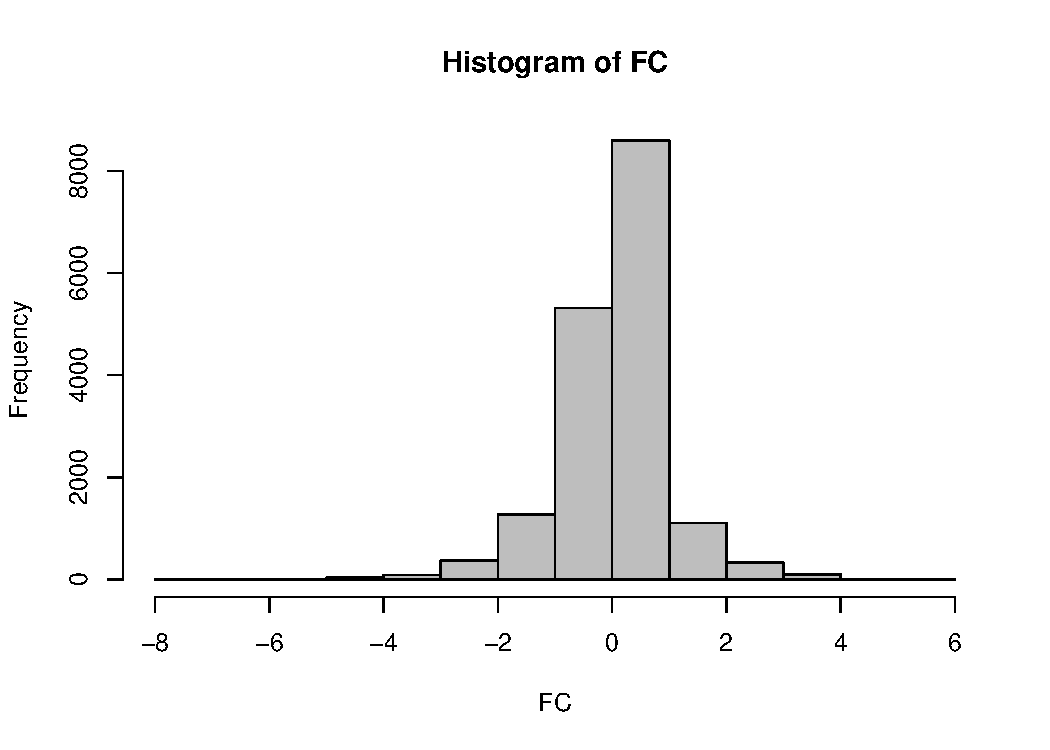
\includegraphics[width=0.5\columnwidth]{Hist_FC} 
\caption[Histogram of FC]{} % The text in the square bracket is the caption for the list of figures while the text in the curly brackets is the figure caption
\label{fig:1} 
\end{figure}
Another criterion to find differentially expressed genes is to use Student’s t test for two conditions.
So we used a t-test to calculate the p-value.
%\begin{figure}[h!]
%\centering 
%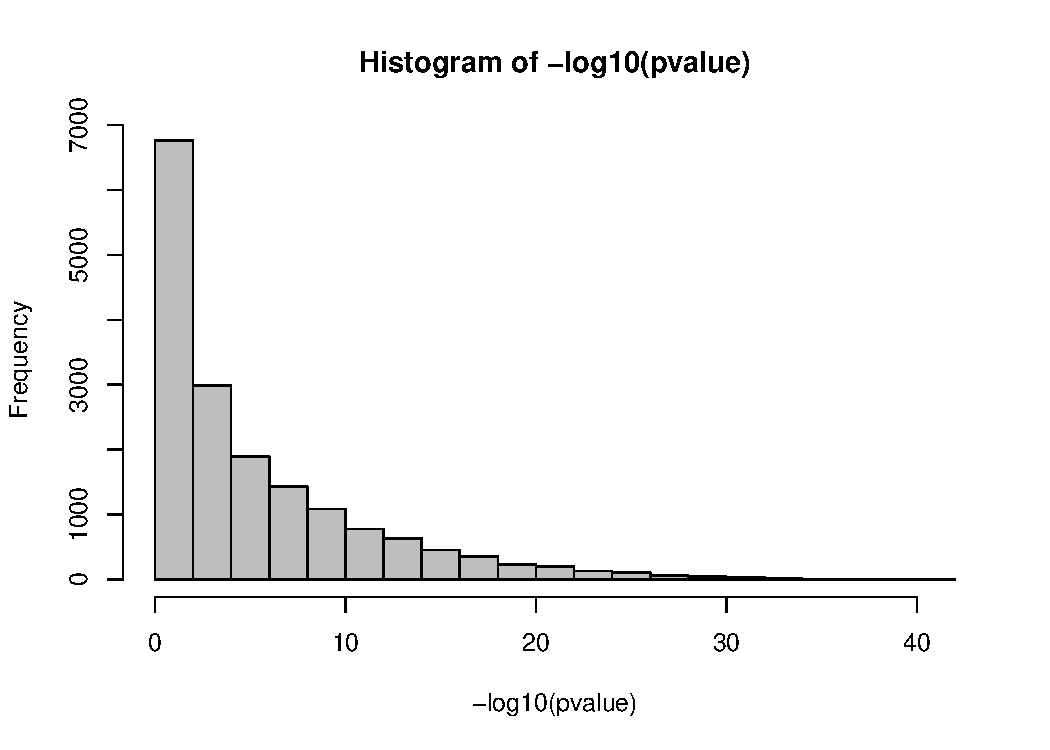
\includegraphics[width=0.6\columnwidth]{Hist_pvalue} 
%\caption[Histogram of $-\log{pvalue}$]{} % The text in the square bracket is the caption for the list of figures while the text in the curly brackets is the figure caption
%\label{fig:1} 
%\end{figure}
We applied the "fdr" method for correction multiple comparison. 
The values obtained are shown on the following histogram (Figure~\ref{fig:2}).

\begin{figure}[!h]
\centering 
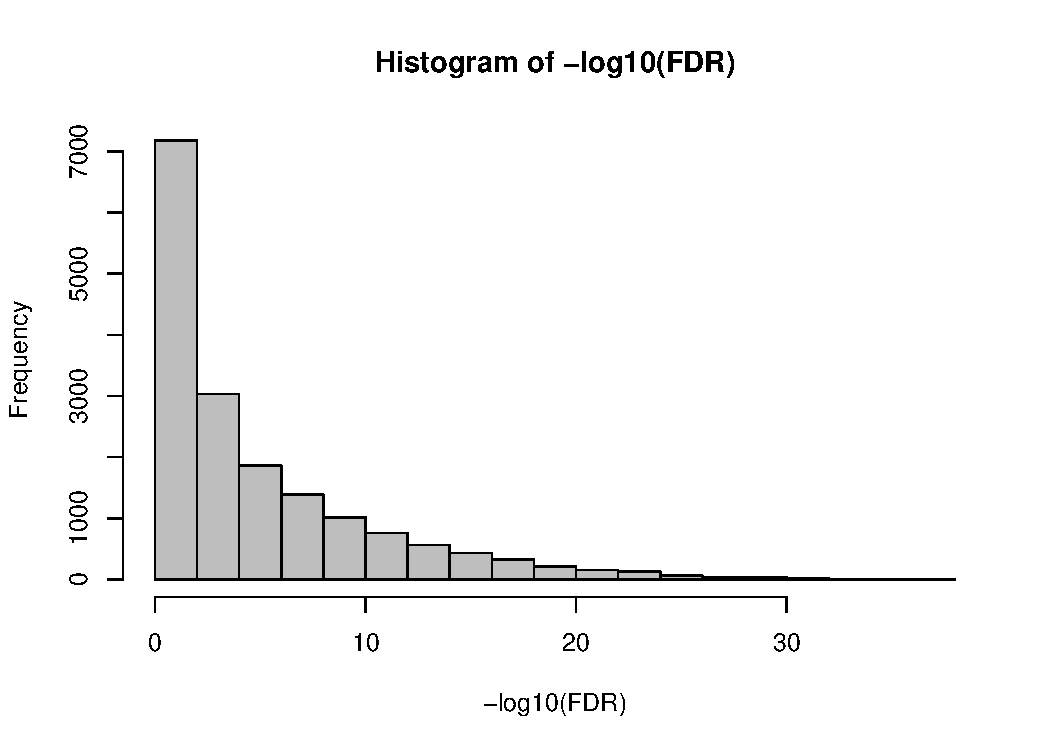
\includegraphics[width=0.5\columnwidth]{Hist_FDR} 
\caption[Histogram of $-\log{(FDR)}$]{} % The text in the square bracket is the caption for the list of figures while the text in the curly brackets is the figure caption
\label{fig:2} 
\end{figure}

We have selected  $|$ fold change$\, | \ge 2.5$ and $fdr \le 0.05$ as threshold values. The result is the volcano plot in Figure~\ref{fig:3}.

\begin{figure}[!h]
\centering 
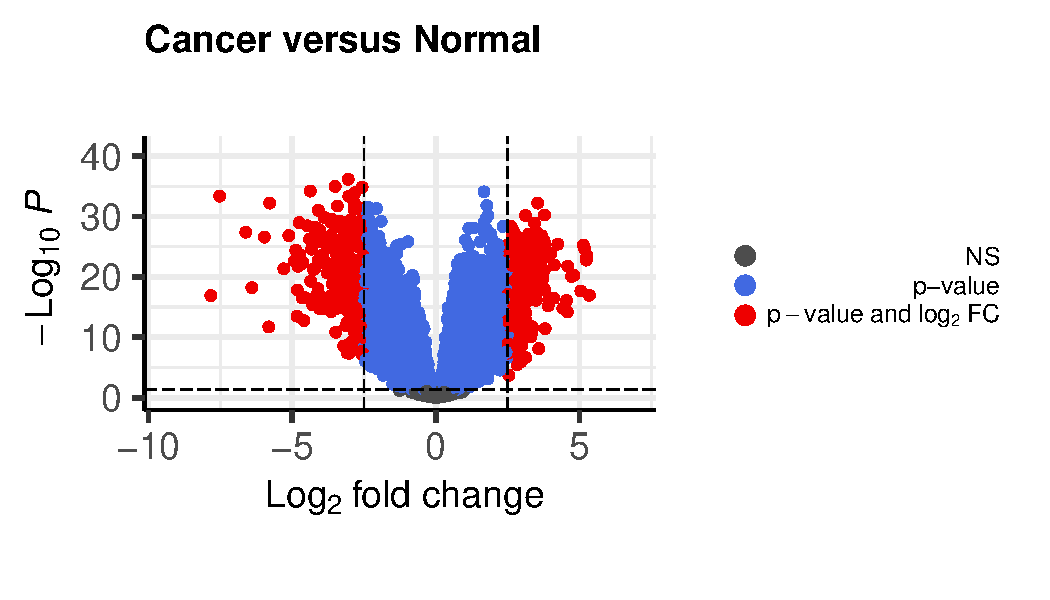
\includegraphics[width=1\columnwidth]{VolcanoDEGs} 
\caption[Volcano Plot]{} % The text in the square bracket is the caption for the list of figures while the text in the curly brackets is the figure caption
\label{fig:3} 
\end{figure}

In the end $494$ genes ($237$ upregulated and $257$ downregulated genes) were found.

% Co-NET------------------------------------------------

\subsection{Co-expression networks}


\begin{figure}[!h]
\centering
\subfloat[Co-expression network in normal cells]{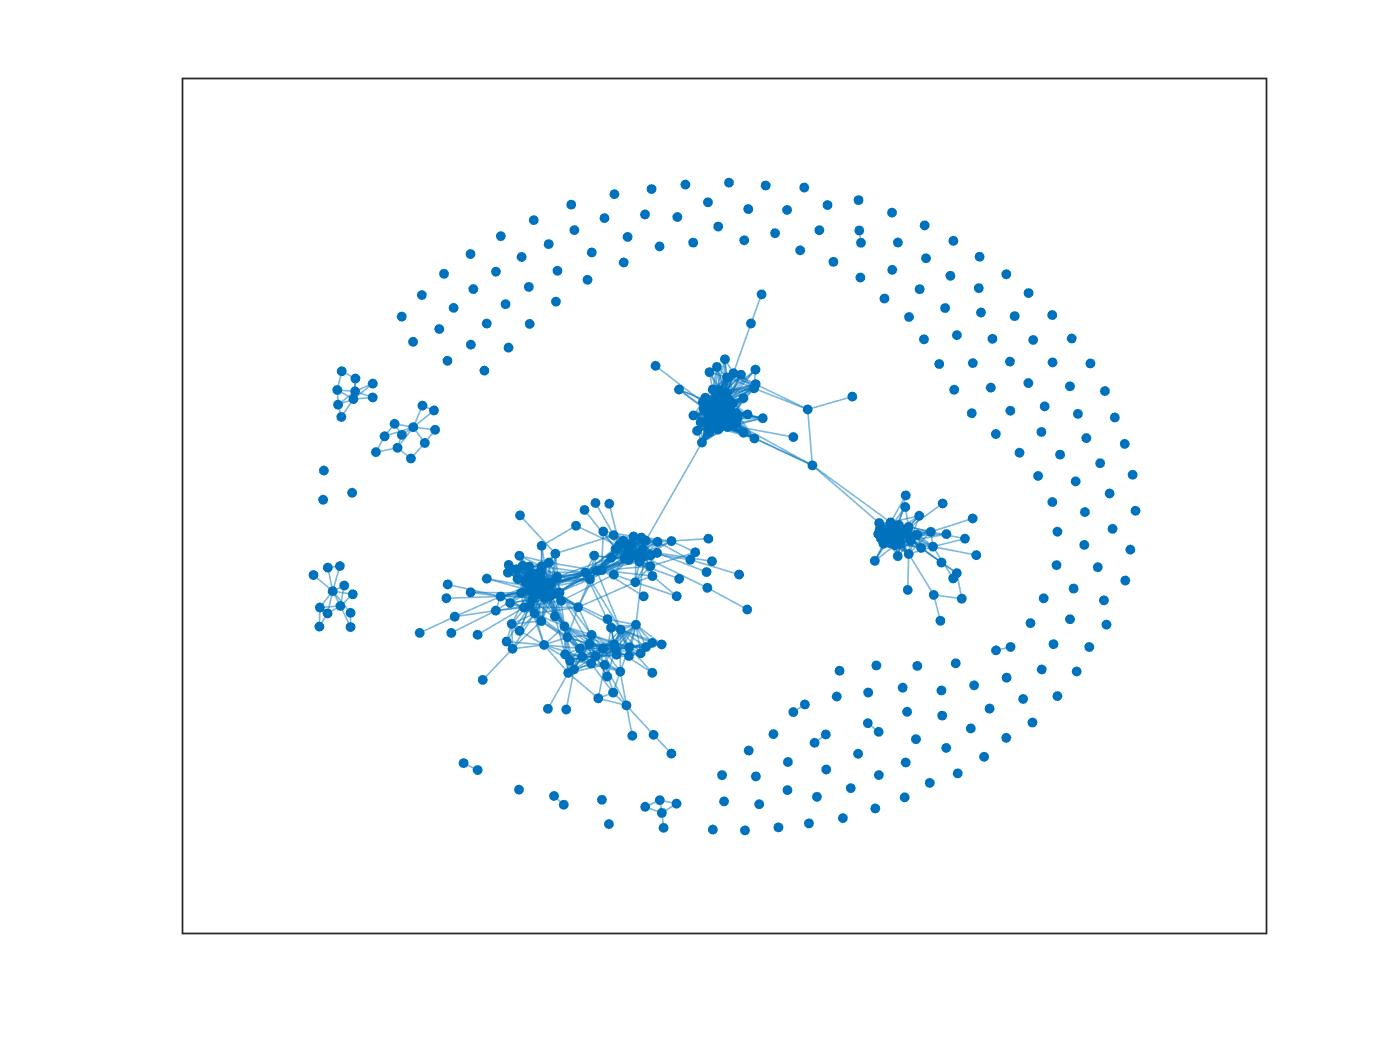
\includegraphics[width=.45\columnwidth]{co-net_N.jpg}} \quad
\subfloat[Co-expression network in cancer cells]{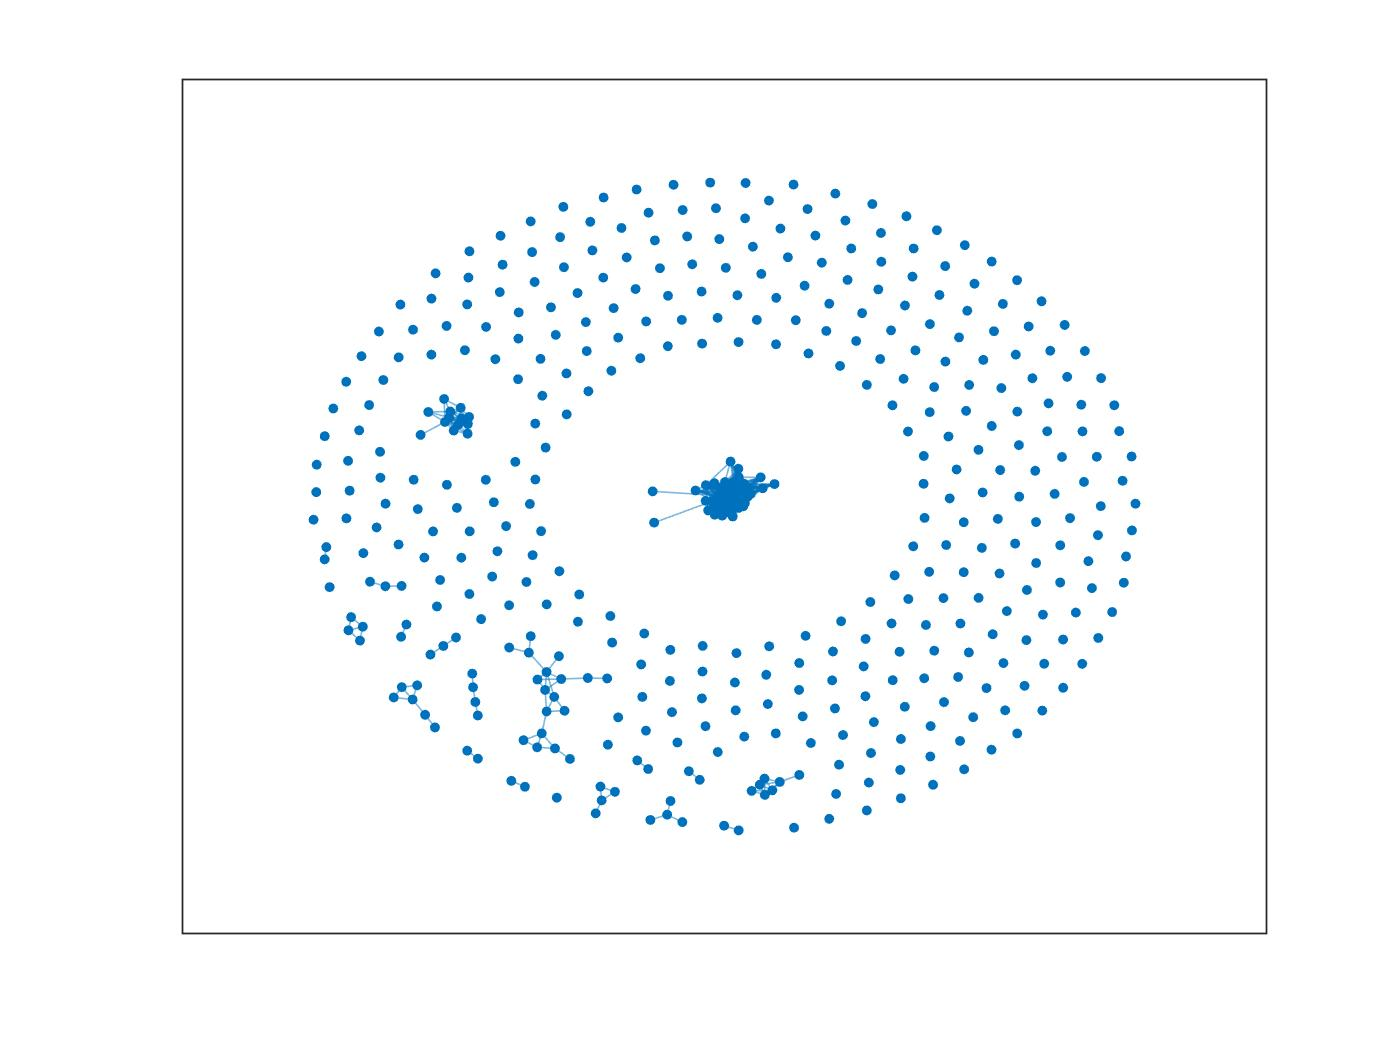
\includegraphics[width=.45\columnwidth]{co-net_C.jpg}\label{fig:ipsum}} 
\caption[Co-expression network in normal and cancer cells]{Co-expression network in normal and cancer cells} % The text in the square bracket is the caption for the list of figures while the text in the curly brackets is the figure caption
\label{fig:esempio}
\end{figure}

\newpage
% Differential Co-NET------------------------------------------------

\subsection{Differential Co-expressed Network}
Instead of establishing that co-expression is significant in one condition and not in the other, we are now going to test directly if the change in co-expression is significant using differential networks: they encode changes in the connections among nodes between the conditions or states.\\

To calculate the differential correlations, first we have stabilized the variance  of sample correlation coefficients in each condition applying the following Fisher z-transformation:

$$
z_{1 \text{or} 2} = \frac{1}{2}\log{\Bigl(\frac{1+\rho_{1 \text{or} 2}}{1-\rho_{1 \text{or} 2}}\Bigr)}
$$

then we compute z-scores to evaluate the correlation:

$$
Z = \frac{z_1 - z_2}{\sqrt{\frac{1}{n_1 - 3}+\frac{1}{n_2 - 3}}}
$$

where $n_1$ and $n_2$ represent the sample size for each of the conditions. Finally we set $|Z|> 5$ as threshold; we get the graph of the Figure~\ref{fig:5}.
\begin{figure}[!h]
\centering 
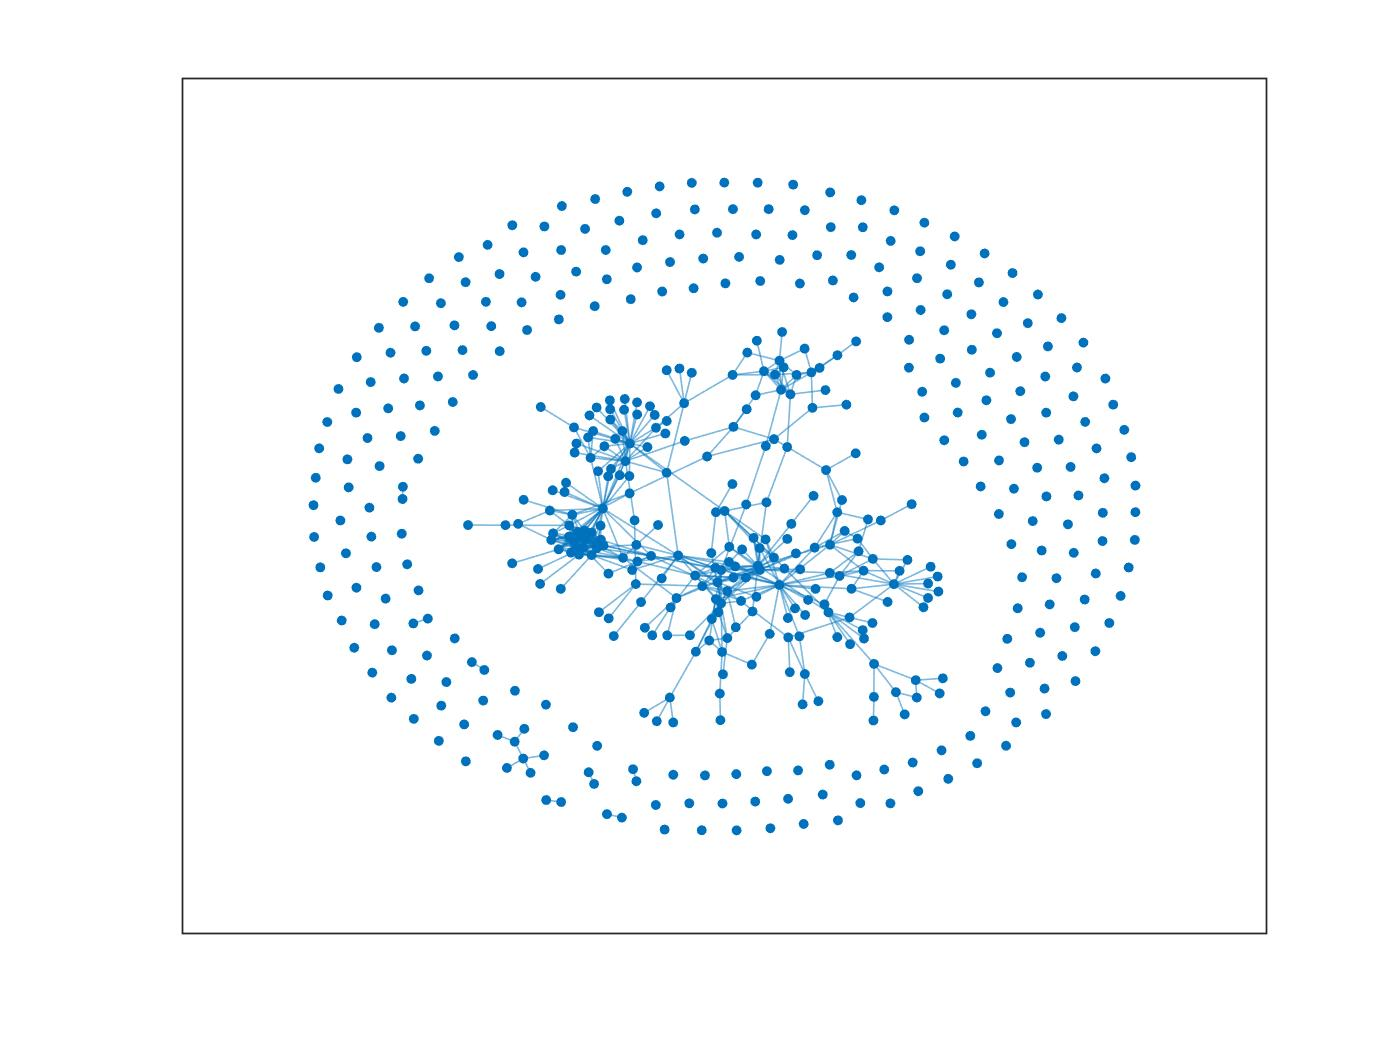
\includegraphics[width=0.6\columnwidth]{diff-co-net} 
\caption[Differentially Co-expression network]{Differentially Co-expression network} % The text in the square bracket is the caption for the list of figures while the text in the curly brackets is the figure caption
\label{fig:5} 
\end{figure}

\begin{figure}[!h]
\centering 
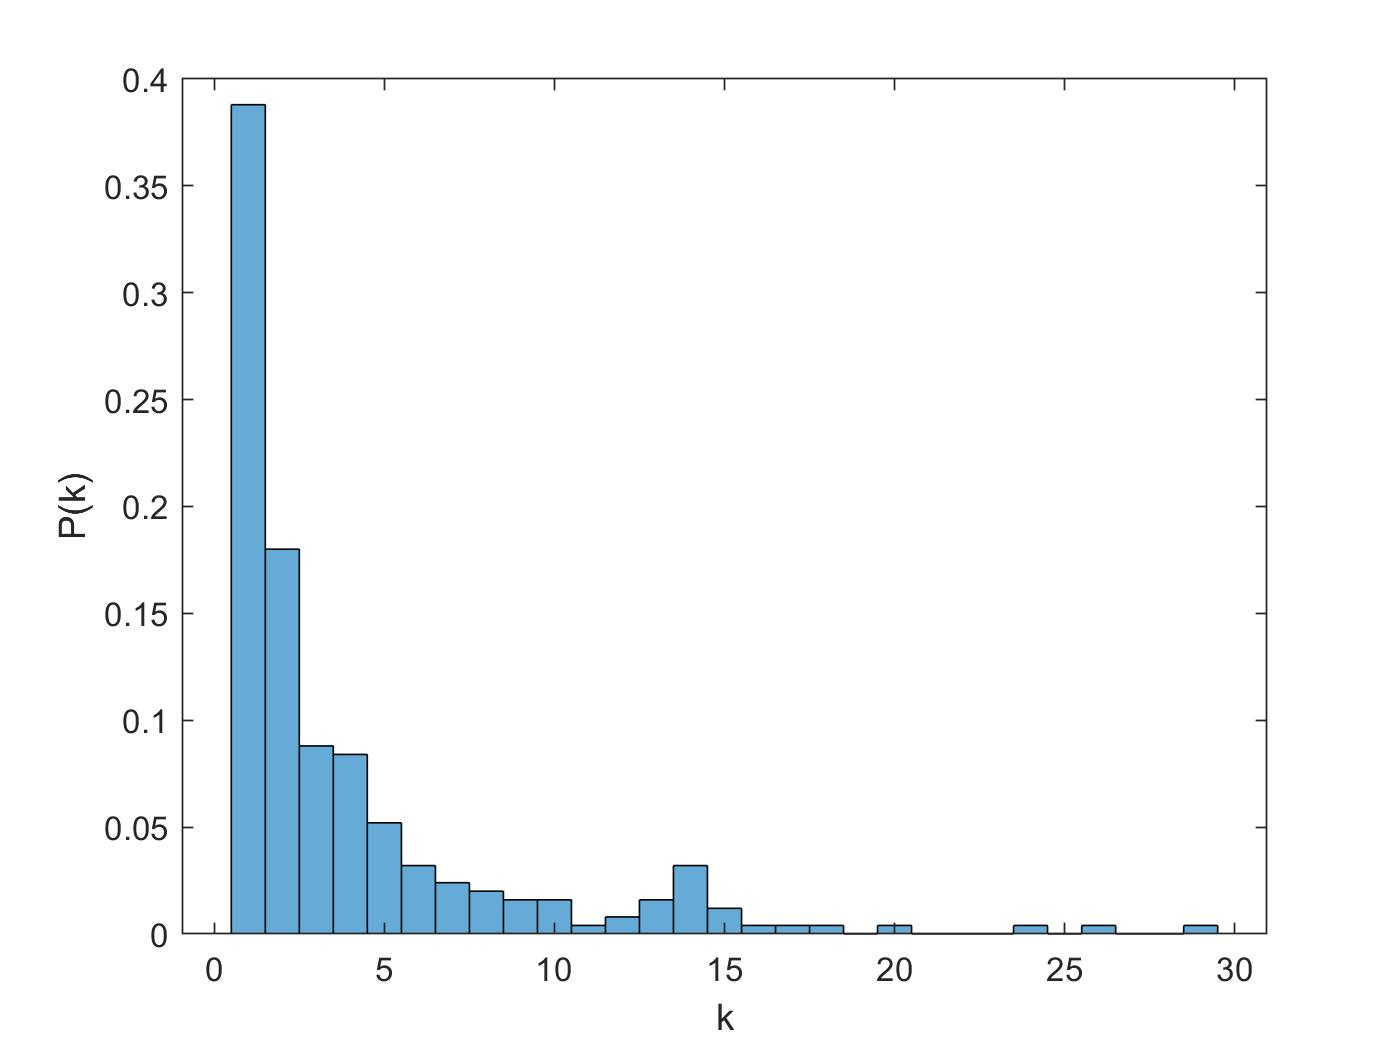
\includegraphics[width=0.6\columnwidth]{diff-co-net_deg_distr} 
\caption[Differentially Co-expression network Degree Distribution]{Differentially Co-expression network Degree Distribution} % The text in the square bracket is the caption for the list of figures while the text in the curly brackets is the figure caption
\label{fig:6} 
\end{figure}

\begin{figure}[!h]
\centering
\subfloat[Degree]{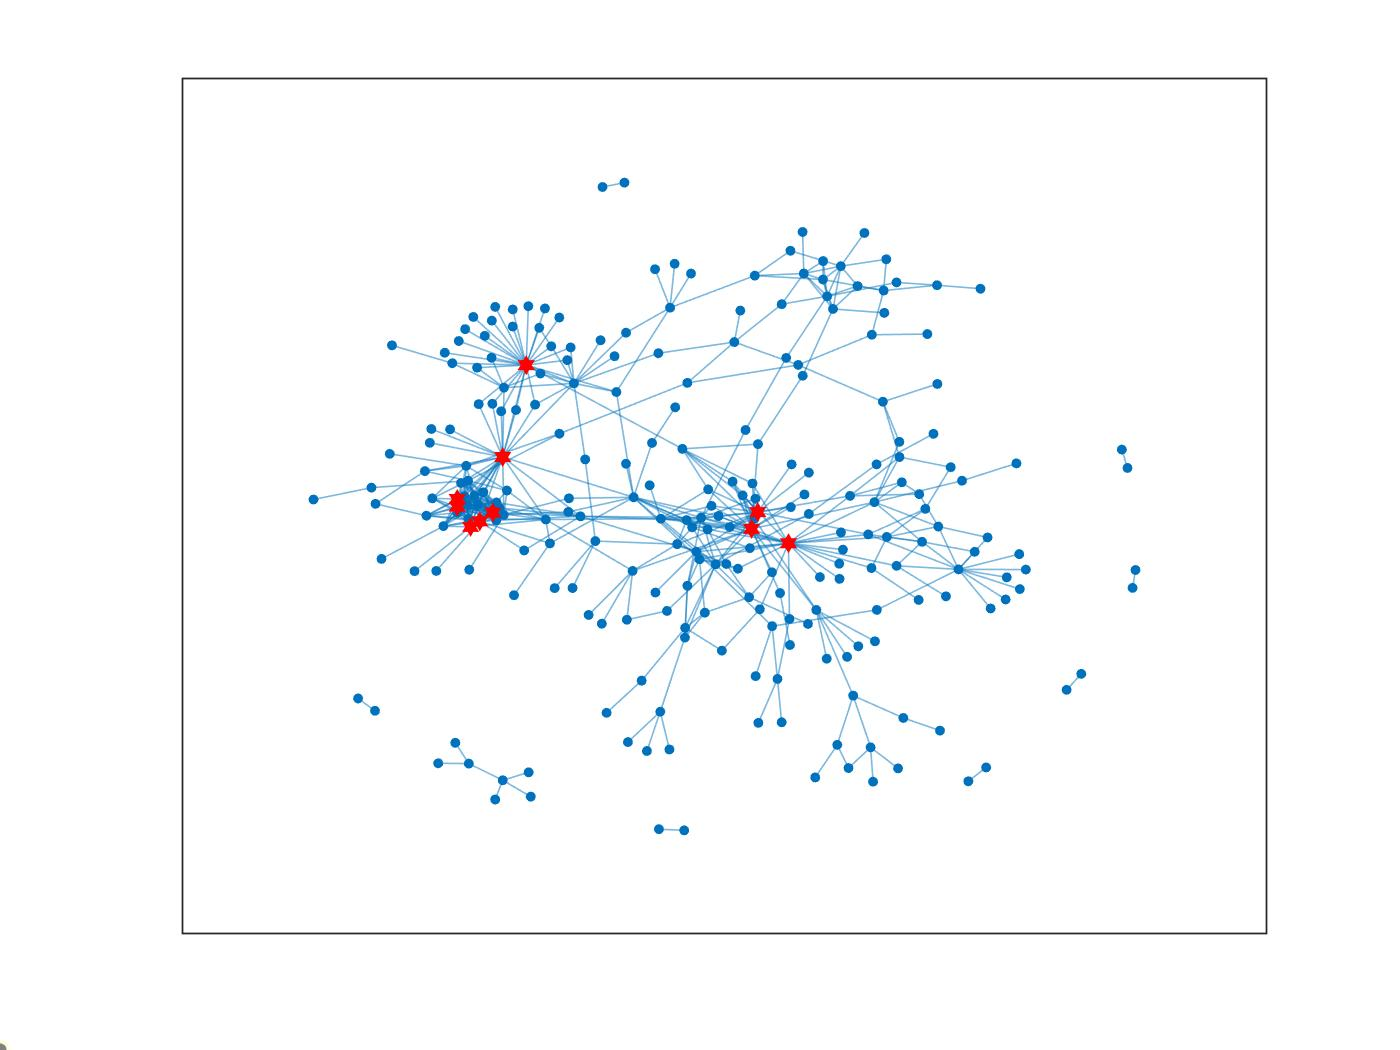
\includegraphics[width=.45\columnwidth]{diff-co-net_degree.jpg}} \quad
\subfloat[Closeness]{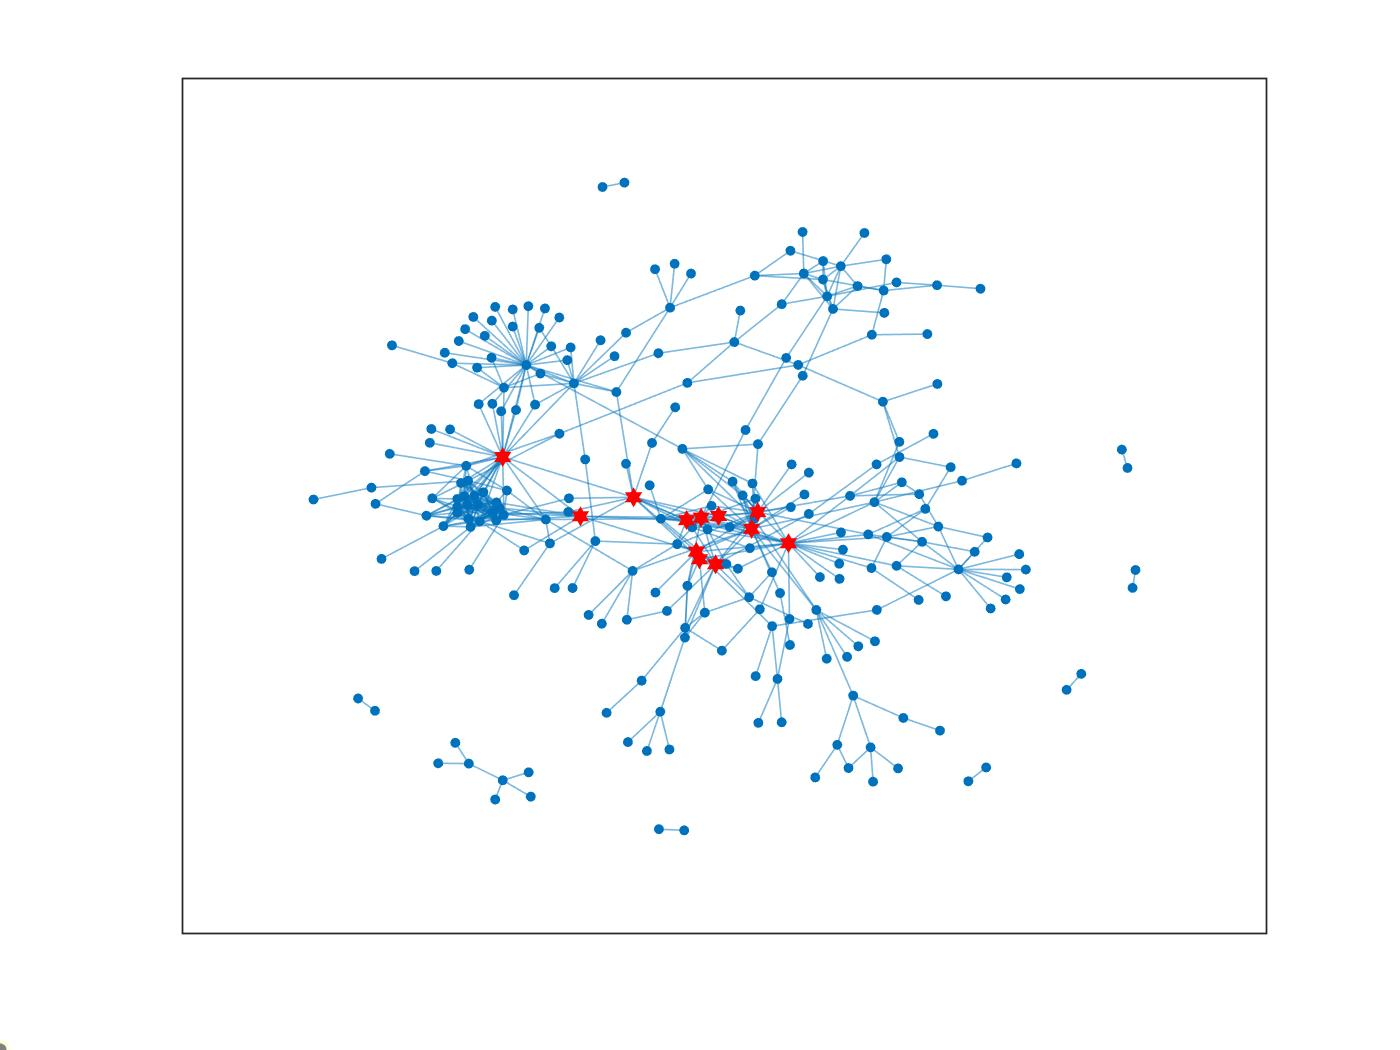
\includegraphics[width=.45\columnwidth]{diff-co-net_closeness.jpg}\label{fig:ipsum}} \\
\subfloat[Betweenness]{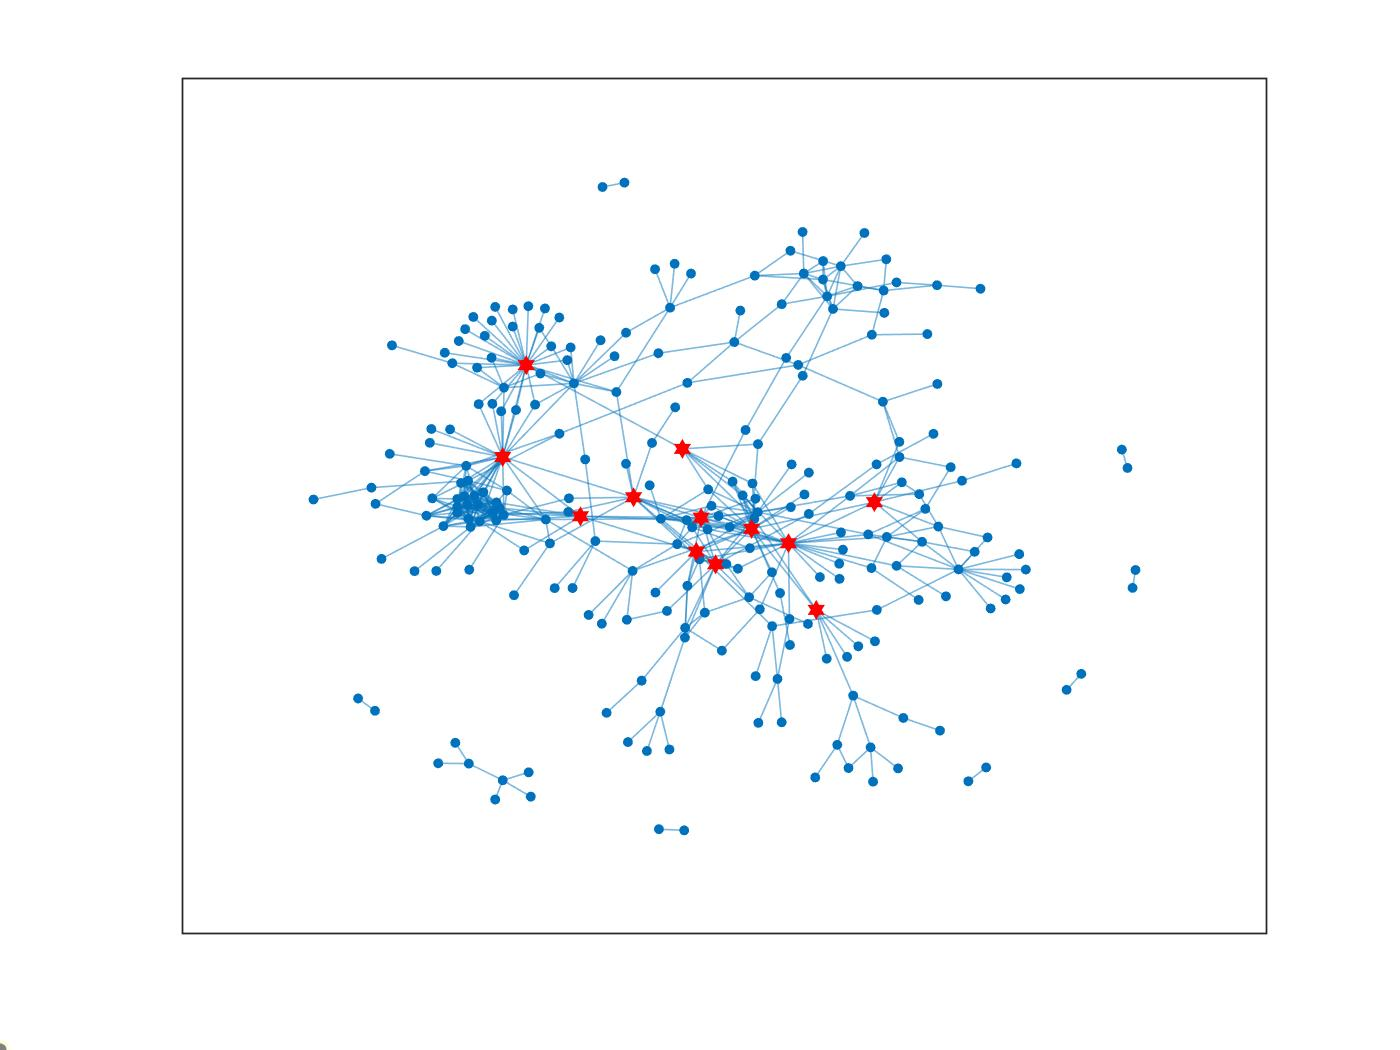
\includegraphics[width=.45\columnwidth]{diff-co-net_betweenness.jpg}} \quad
\subfloat[Eighenvector]{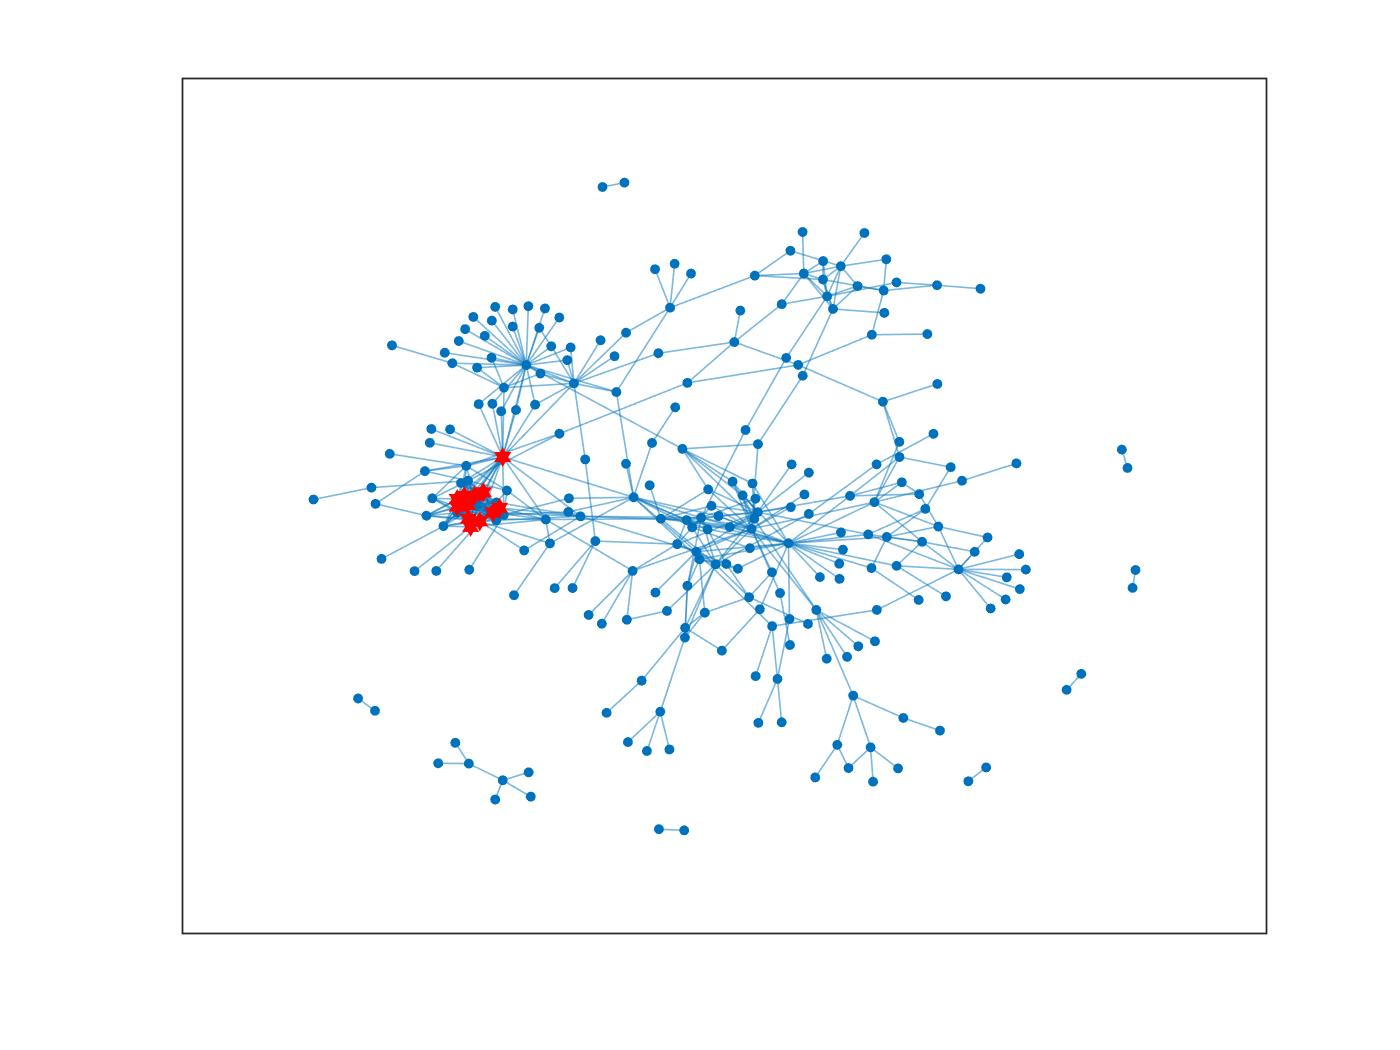
\includegraphics[width=.45\columnwidth]{diff-co-net_eigenvector.jpg}}
\caption[Centrality Measures Differential Co-Net]{Centrality Measures} % The text in the square bracket is the caption for the list of figures while the text in the curly brackets is the figure caption
\label{fig:esempio}
\end{figure}

\newpage
%----------------------------------------------------------------------------------------
%	RESULTS AND DISCUSSION
%----------------------------------------------------------------------------------------

\section{Results and Discussion}
\begin{figure}[!h]
\centering 
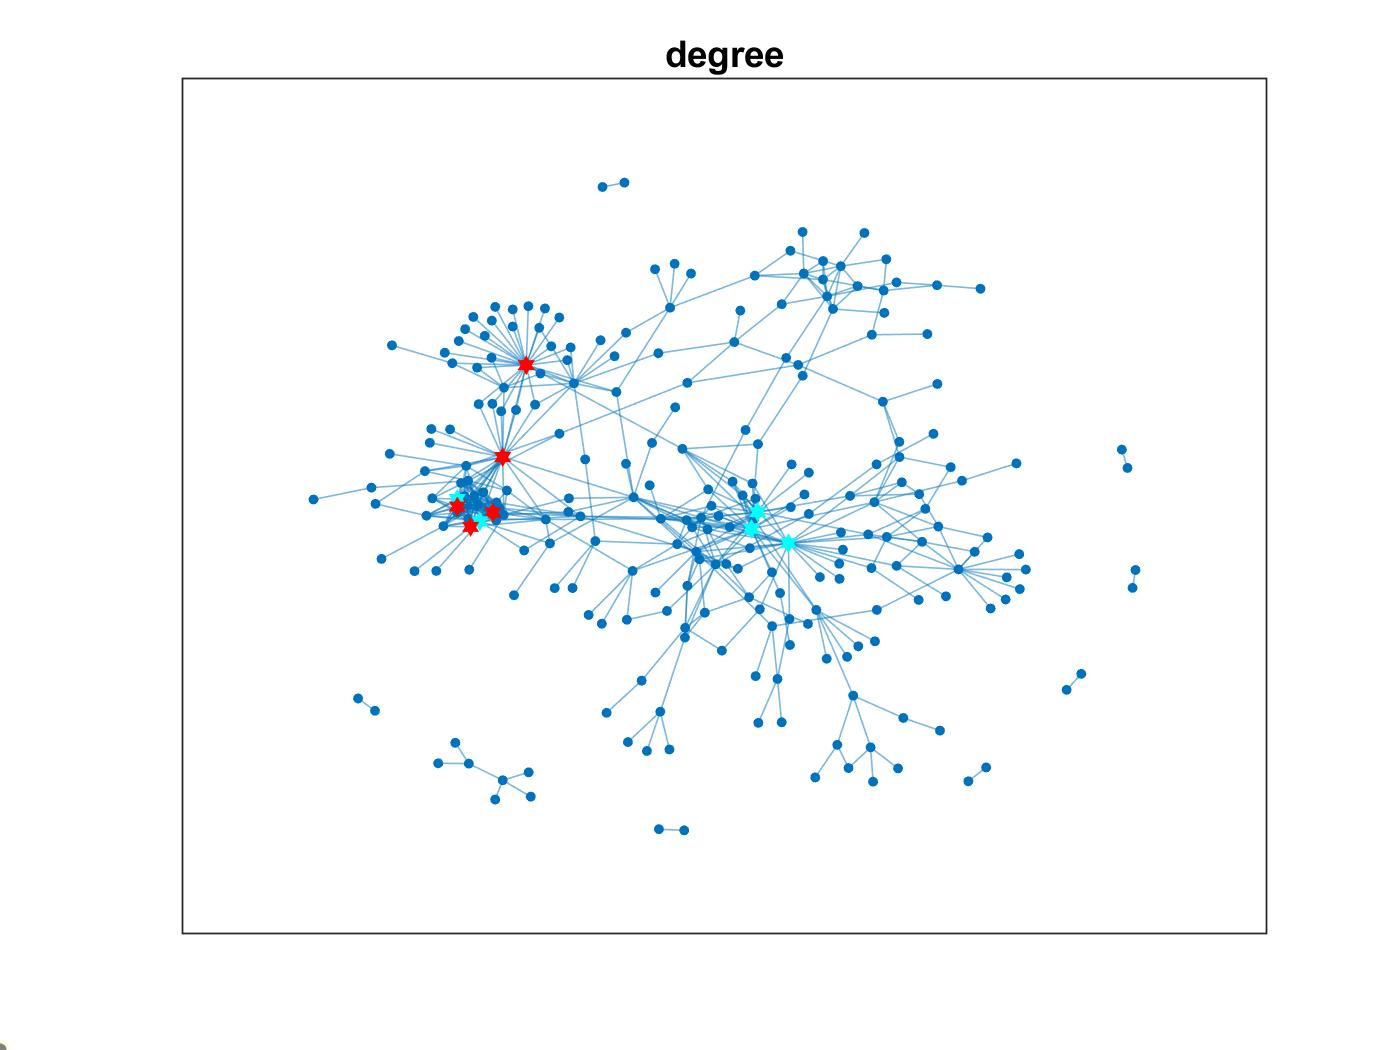
\includegraphics[width=0.6\columnwidth]{diff-co-net_compare_hub_sets} 
\caption[Differentially Co-expression network compare hub sets]{Differentially Co-expression network compare hub sets} % The text in the square bracket is the caption for the list of figures while the text in the curly brackets is the figure caption
\label{fig:7} 
\end{figure}



\newpage
%----------------------------------------------------------------------------------------
%	BIBLIOGRAPHY
%----------------------------------------------------------------------------------------

\renewcommand{\refname}{\spacedlowsmallcaps{References}} % For modifying the bibliography heading

\bibliographystyle{unsrt}

\bibliography{sample.bib} % The file containing the bibliography

%----------------------------------------------------------------------------------------

\end{document}